\documentclass[11pt,a4paper]{article}

% 调整页边距
\usepackage{geometry}
\geometry{a4paper,scale=0.82}

\usepackage{graphicx} %插入图片的宏包
\usepackage{float} %设置图片浮动位置的宏包
\usepackage{subfigure} %插入多图时用子图显示的宏包

\begin{document}

\title{Pattern Recognition Assignment 1}
\author{2031566 - Han Yang \\
{\small{hanyang\_sh@tongji.edu.cn}}
}
\date{\today}
\maketitle

\section{Dataset}
I choose the dataset Horse Colic \footnote{http://archive.ics.uci.edu/ml/datasets/Horse+Colic} from UCI Machine Learning Repository.
This dataset contain 300 training instances and 68 test instances. It has 28 attributes, such as rectal temperature and pulse and 
respiratory rate, with  30\% of the values are missing. As for this assignment, I use rectal temperature and pulse. Rectal temperature
is linear and in degrees celsius, may be reduced when the animal is in late shock, normal temp is 37.8. Pulse is the heart rate in
beats per minute, 30 -40 is normal for adults, animals with painful lesions or suffering from circulatory shock may have an elevated 
heart rate. With those attributes, We can train a clssifier to predict whether the horse will survive.


\section{Preprocess}
As there exist 30\% missing value, there are many ways to deal with it, for this assignment i just drop the incorrect instances. In the
origin data, the outcome attribute hava three types(1 2 3)mean lived died and euthanized. For the binary logistic regression, we can
only classify two classes, so i classify euthanasia and death into one category denoted by 1, and live denoted by 0.

\section{Modules}

    \subsection{Preprocess}
        As description above, we need to preprocess the original data, I use numpy and pandas to process the data and save processed
        data to csv format.
    
    \subsection{Logistic Regression Algorithm}
        The main part of logistic regression is the logistic function (sigmoid function) and probability function and cost function, I
        augment $X$ to $X=(X;1)$ and $w$ dimension to feature number plus 1:
            $$ Sigmoid\ Function : g(z) = \frac{1}{ 1 + e^-z } \eqno{1.1} $$
            $$ Hypothesis \ Function: h(X) = g(X \omega) \eqno{1.2} $$
            $$ Cost\ Function: J(\omega) = -\frac{1}{m} \sum \left( Y \log h(X) + (1 - Y ) \log (1-h(X)) \right) \eqno{1.3} $$
        Instead of using Newton's Methos showed in the slide, I use Gradient Descent to optimize this minmiun problem. Use the following
        formulas to get derivative of $\omega$:
            $$ \frac{\partial J(\omega) }{\partial \omega} = \frac{1}{n} X^T (h(X) - y) \eqno{{1.4}}$$

    \subsection{Plot}
        After 4000 iterations, we have get the augmented $\omega = [-0.07633064 , 0.03203682 , 0.00125518] ^ T$ , and i use matplotlib
        to plot the decision boundary.

\section{Result}
    This dataset is not well,i use the hyperparameter at $learning\_rate = 1e-5, num\_iterations = 4000$ and I get a result at
    $\omega=[-0.07633064 , 0.03203682 , 0.00125518] ^ T, train\_accurancy = 0.6837606837606838, test\_accurancy = 0.728813559322034 $. And I plot the decision boundary in Figure \ref{Fig.main2} and cost curve in Figure \ref{Fig.main3}.

    \begin{figure}[H]
        \centering
        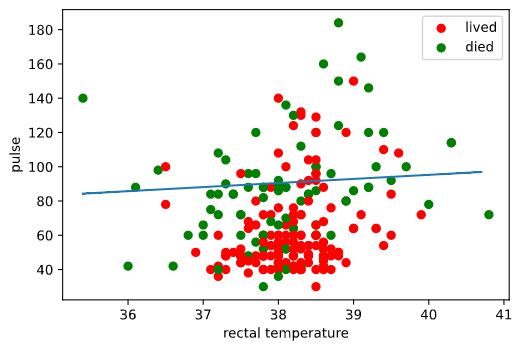
\includegraphics[width=0.6\textwidth]{Figure_2.png} %插入图片,[]中设置图片大小,{}中是图片文件名
        \caption{Decision boundary}
        \label{Fig.main2}
    \end{figure}

    \begin{figure}[H]
        \centering
        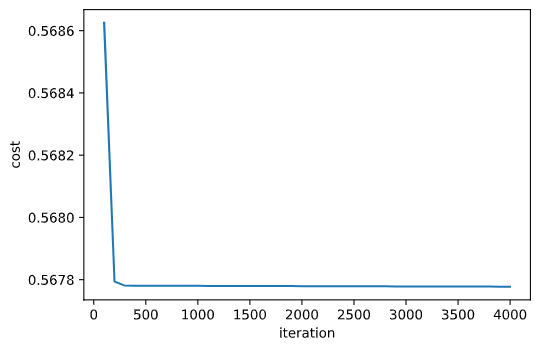
\includegraphics[width=0.6\textwidth]{Figure_3.png} %插入图片,[]中设置图片大小,{}中是图片文件名
        \caption{Cost curve}
        \label{Fig.main3}
    \end{figure}

    The horse dataset is linearly inseparable, to get a better result, I use the Iris dataset\footnote{http://archive.ics.uci.edu/ml/datasets/Iris} to do this assignment 
    again. I use the hyperparameter at $learning\_rate = 1e-4, num\_iterations = 4000$ and I get a
    result: $W = [ 0.95465512 ,-1.64464035, -0.17745044]^T, train\_accurancy = 0.9875,
    test\_accurancy = 1.0$.And I plot the decision boundary in Figure \ref{Fig.main4} and cost curve in Figure \ref{Fig.main5}.

    \begin{figure}[H]
        \centering
        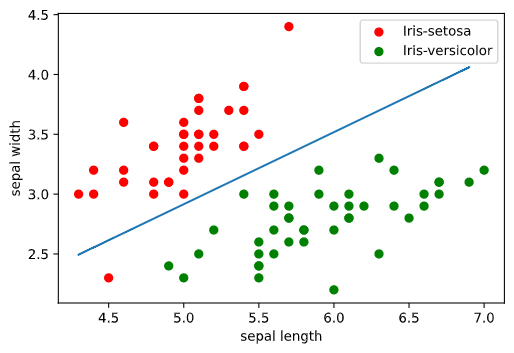
\includegraphics[width=0.6\textwidth]{Figure4.png} %插入图片,[]中设置图片大小,{}中是图片文件名
        \caption{Decision boundary}
        \label{Fig.main4}
    \end{figure}

    \begin{figure}[H]
        \centering
        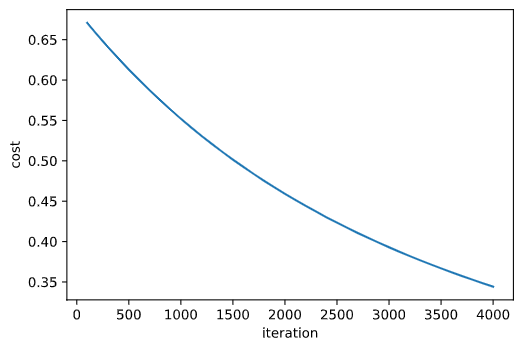
\includegraphics[width=0.6\textwidth]{Figure5.png} %插入图片,[]中设置图片大小,{}中是图片文件名
        \caption{Cost curve}
        \label{Fig.main5}
    \end{figure}

\end{document}
